\chapter{Diseño}
\label{cap:capitulo4}

\begin{flushright}
\begin{minipage}[]{9cm}
\emph{El diseño no es solo lo que se ve y lo que se siente. El diseño es cómo funciona.}\\
\end{minipage}\\

Steve Jobs, \textit{conferencia de lanzamiento del Apple iPod, 2001}\\
\end{flushright}

\vspace{1cm}

Después de definir la plataforma de desarrollo, se procede a explicar el diseño de la aplicación.

El sistema está diseñado para gestionar la rehabilitación motora de pacientes post-ictus mediante la interacción con un brazo robótico.
Esto se lleva a cabo a través de una aplicación que controla diversos parámetros que afectan a la trayectoria, las perturbaciones y nivel de asistencia del brazo.
A continuación, se definen los puntos clave del sistema:
\begin{itemize}
    \item Trayectoria: representa el recorrido deseado que el paciente debe seguir durante la terapia. Es una señal definida por los parámetros de frecuencia, amplitud y tipo de señal (trayecto constante o dinámico). El objetivo es medir la precisión del paciente al seguir la trayectoria.
	\item Perturbación: es una señal que altera la trayectoria. Se define mediante los parámetros de amplitud, duración y tipo (perturbación escalón o sinusoidal). El objetivo es proporcionar un desafío adicional al paciente.
	\item Límites: definen las restricciones físicas de movilidad del brazo robótico. Se establecen un límite inferior (mínimo) y superior (máximo), así como un offset que determina la posición inicial del brazo. Se ajustan llevando el brazo a la posición deseada.
	\item Asistencia: se refiere al grado de apoyo que ofrece el brazo robótico al paciente. Este parámetro se ajusta tanto de forma dinámica, según el nivel de dificultad del juego, como manual, a través de la interfaz de control.
	\item Nivel de dificultad: hace referencia al nivel de dificultad del juego. El nivel de dificultad aumenta de forma progresiva, reduciendo el nivel de asistencia del robot. Puede ajustarse tanto dinámicamente como manualmente al igual que la asistencia.\\
\end{itemize}\

Más adelante, se describen los nodos y topics utilizados en la plataforma.

\section{Esquema de nodos y topics}
\label{section:review}

En la Imagen \ref{fig:nodes} se contempla un esquema de los nodos, topics y tipos de datos que se utilizan para la comunicación de la plataforma software con el actuador.

\begin{figure}[ht!]
	\centering
	\begin{minipage}{1.0\linewidth}
		\centering
		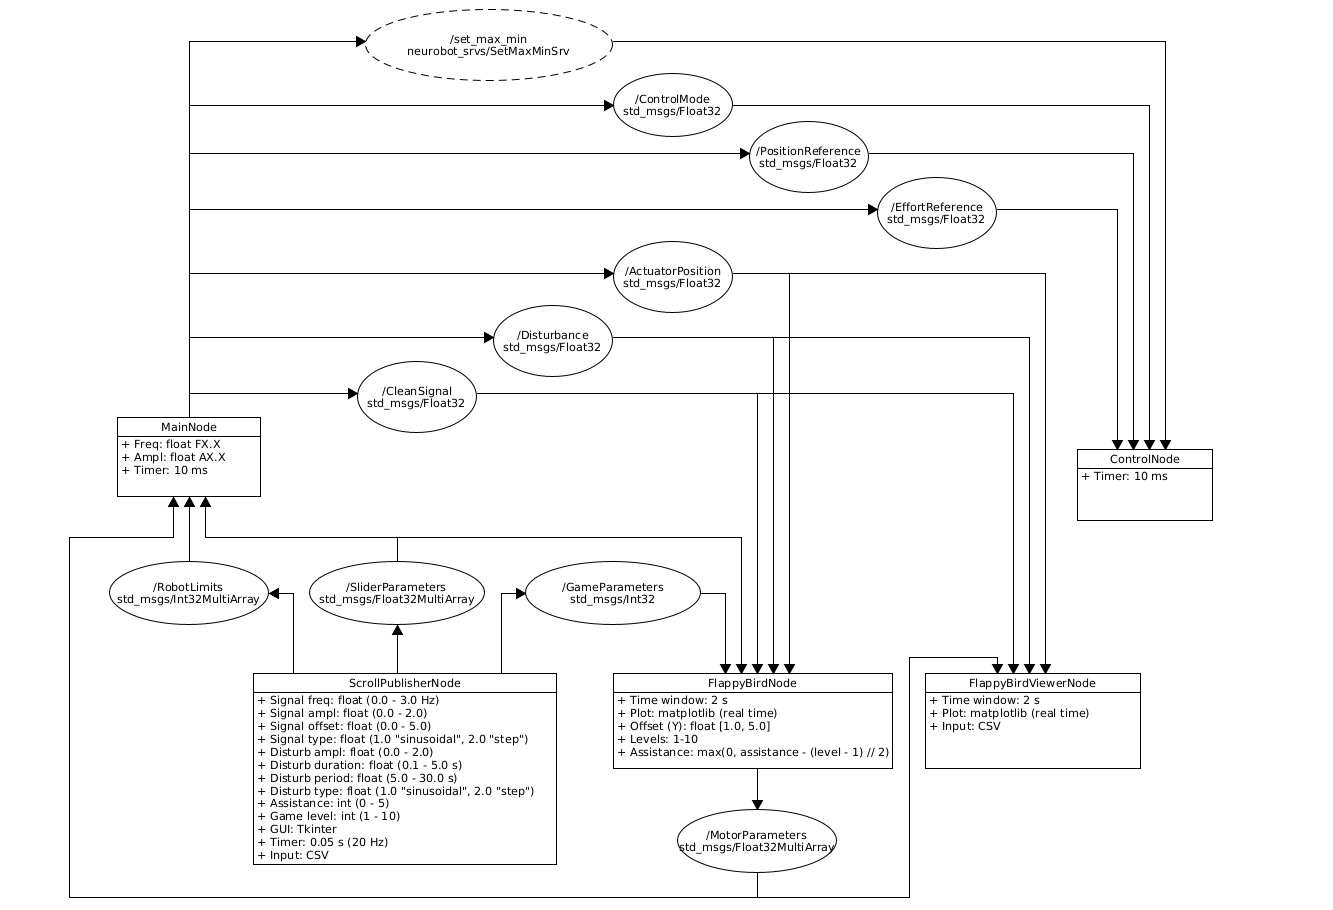
\includegraphics[width=\linewidth]{figs/esquema_nodos.png}
	\end{minipage}
	\caption[Esquema de nodos y topics]{Esquema de nodos y topics}
	\label{fig:nodes}
\end{figure}

Seguidamente, se detalla la función de los nodo y la información trasmitida por cada uno de los topics:
\begin{itemize}
    \item \verb|LimitNode|: este nodo gestiona la configuración de los límites del brazo robótico. Utiliza el topic \verb|/RobotLimits|, como un booleano para indicar el límite que se ajusta.
	\item \verb|ScrollPublisherNode|: este nodo publica los parámetros de la trayectoria y la perturbación en el topic \verb|/SliderParameters|, y del juego (asistencia y nivel de dificultad) en \verb|/GameParameters|. La actualización de los datos se realiza cada $50 ms$.
	\item \verb|FlappyBirdNode|: este nodo implementa la lógica del juego basado en seguir una trayectoria o mantener una posición. Recibe la señal de referencia del topic \verb|/CleanSignal|, la señal de perturbación de \verb|/Disturbance|, la asistencia y nivel de dificultad de \verb|/GameParameters|, los límites y el offset de \verb|/SliderParameters| y la posición del jugador de \verb|/ActuatorPosition|. Y publica los datos de referencia de las señales y tiempo, en el momento de la posición del jugador en el eje X, en el topic \verb|/MotorParameters|. La actualización de los datos se realiza cada $10 ms$.
	\item \verb|FlappyBirdViewerNode|: este nodo grafica las señales de trayectoria, perturbación y la posición del paciente, que recibe de los topics \verb|/CleanSignal|, \verb|/Disturbance| y \verb|/ActuatorPosition|, respectivamente, para visualizar el progreso del paciente durante la terapia. Además, calcula el error de posición a través de los datos publicados en el topic \verb|/MotorParameters|, explicados en el nodo anterior.\\
\end{itemize}\

El proyecto se divide en cuatro scripts, el primero se utiliza para crear o registrar un paciente, el segundo lanza la GUI y controla los parámetros del juego, el tercero permite visualizar el comportamiento del paciente durante la terapia, y el cuarto es el propio juego.

\section{Interfaz de registro de un paciente}
\label{section:registro}

Este script permite gestionar un conjunto de datos, que registran a un paciente, mediante una GUI.

En primer lugar, se importan las bibliotecas estándar, mencionadas en el capítulo anterior, como \verb|tkinter|, que se utiliza para crear la interfaz gráfica, \verb|csv| para guardar los datos en un archivo CSV para su posterior uso, y \verb|os| para interactuar con el sistema de archivos.

Se obtiene el directorio de inicio del usuario y se crea un directorio dentro de este, si no existe, bajo el nombre \textit{database}, donde se almacenan los ficheros con los datos de registro y análisis terapéuticos de cada paciente.

Se definen tres funciones principales que gestionan las operaciones de la GUI.
La función \verb|exit()| cierra la ventana principal de Tkinter, \verb|clear()| limpia los campos de entrada y texto, y \verb|savedata()| guarda los valores de los campos, valida que el ID sea un número y crea un subdirectorio bajo el nombre del ID, si no existe, donde guarda los datos en un archivo CSV llamado \verb|ID.csv|.
Si el archivo no existe, se escribe el encabezado utilizando \verb|writer.writeheader()|.
Los datos se escriben con \verb|csv.DictWriter| y son guardados como \verb|strings|.

Se crea una ventana principal con un título y tamaño fijo de $600x500$ píxeles.
Los estilos visuales se configuran con \verb|ttk.Style| y se definen dos frames distintas, \verb|main_frame| se utiliza como contenedor de los campos de entrada y texto y \verb|button_frame| agrupa la lógica de los botones.
Cada campo es un \verb|Entry| enlazado a una variable de tipo \verb|StringVar| y hacen referencia al nombre, apellido e ID del paciente, frecuencia, amplitud y perturbación de la señal que generará el brazo robótico, nivel y progreso del juego y un espacio para que el doctor incluya observaciones.
Se crean dos botones, \textit{Save} llama a \verb|savedata()| para guardar los datos, que a su vez llama a \verb|clear()| para limpiar los campos una vez que estos se han almacenado, y el botón \textit{Exit} llama a la función \verb|exit()| que cierra la aplicación.
En la Imagen \ref{fig:database} puede observarse el estilo de la interfaz.

\begin{figure}[ht!]
	\centering
	\begin{minipage}{0.65\linewidth}
		\centering
		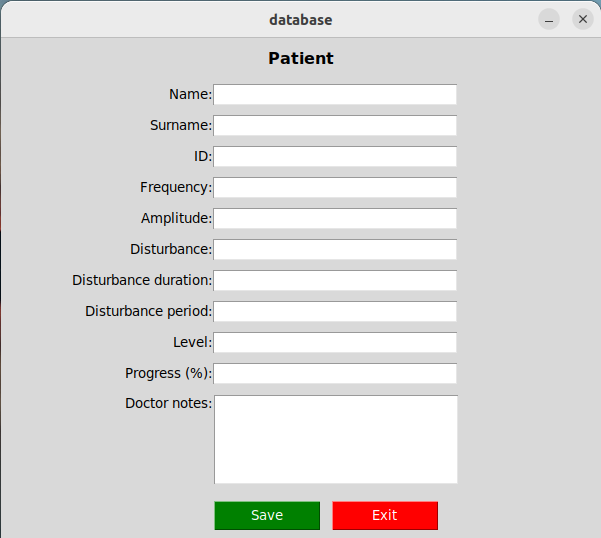
\includegraphics[width=\linewidth]{figs/registro.png}
	\end{minipage}
	\caption[Interfaz de registro de un paciente]{Interfaz de registro de un paciente}
	\label{fig:database}
\end{figure}

\verb|root.mainloop()| inicia el bucle de eventos de Tkinter y la interfaz está activa hasta que el usuario cierra la ventana.

\section{Interfaz de control}
\label{section:controller}

Este script combina ROS 2 y Tkinter para crear una GUI que gestiona límites físicos (mínimo, máximo y offset) del robot, adaptándose al brazo específico del paciente que se va a rehabilitar, configura y publica parámetros para crear una señal de control y perturbación para un sistema robótico, parámetros de asistencia y nivel de dificultad para un videojuego terapéutico y almacena dichas configuraciones por paciente.

Al inicio del script se importan las librerías \verb|rclpy| y \verb|std_msgs.msg| para gestionar la comunicación entre Python y ROS 2, \verb|tkinter| para crear la interfaz gráfica, \verb|csv| para el manejo de archivos CSV, \verb|os| para interactuar con el sistema y \verb|datetime| para gestionar la fecha de creación de los archivos.

Se crea un directorio en el directorio de inicio del usuario, si no existe, bajo el nombre \textit{database}, donde se almacenan los ficheros con los datos de configuración de cada paciente.

Se definen dos clases, \verb|ScrollPublisherNode| y \verb|ScrollGUI|.
La primera es una clase de ROS 2 que publica los parámetros de dos señales, de tipo trayectoria y perturbación en el topic \verb|/SliderParameters| y los datos de asistencia y nivel de juego en \verb|/GameParameters|.
Los mensajes son de tipo \verb|Float32MultiArray| y \verb|Int32MultiArray|, y se publican cada $50 ms$ y únicamente cuando se actualiza el valor de los datos, respectivamente.
La decisión de publicar ambas señales en el mismo topic a dicha velocidad se debe a que la actualización de los datos debe realizarse de forma casi instantánea para permitir ajustes inmediatos en los parámetros de la terapia y evaluar la rapidez de respuesta del paciente.
Y, se ha comprobado que esta estimación es lo suficientemente rápida para satisfacer estos requisitos.
Los datos necesarios para generar la señal de trayectoria son frecuencia, amplitud y tipo, mientras que para la perturbación son duración, amplitud y tipo.
El tiempo de las señales se define de manera distinta para evitar redundancias, ya que la perturbación no es constante.
En su lugar, se estima una duración que facilita el entendimiento del terapeuta.
El tipo de señal hace referencia al modo de juego y se codifica como 1.0 (hold o mantener) y 2.0 (follow o seguir), y el tipo de perturbación como 1.0 (sinusoidal) y 2.0 (step o escalón).
También se define un offset que determina la distancia entre la señal principal y los límites superior e inferior, ajustando así los márgenes del camino.
La segunda clase crea la interfaz gráfica y permite ajustar los parámetros del juego en tiempo real y publicarlos a través de un nodo de ROS.
Los datos se guardan en un archivo CSV bajo el nombre \verb|ID-year-month-day-config_<index>.csv| en un subdirectorio llamado \textit{config} dentro del directorio \textit{home/user/database/ID/}.
\verb|index| hace referencia al número de archivo de la sesión diaria.
Si el archivo no existe, se escribe un encabezado con los nombres de los campos a los que hacen referencia los datos como se observa en el Código \ref{cod:codejemplo2}.

\begin{code}[h]
\begin{lstlisting}[language=Python]
header = ["frequency", "amplitude", "offset", "signal", "disturbance", "duration", "period", "mode"]
\end{lstlisting}
\caption[Encabezado del fichero de configuración]{Encabezado del fichero de configuración}
\label{cod:codejemplo2}
\end{code}

Se crean deslizadores, utilizando \verb|ttk.Scale|, para ajustar la frecuencia, amplitud, offset, duración y periodo de las señales, lo que facilita la configuración de los parámetros con mayor precisión y comodidad.
Se utiliza \verb|Combox| para permitir la selección entre los distintos tipos de señal y perturbación y niveles de asistencia (del 0 al 5, donde 0 es asistencia nula y 5 asistencia máxima) y de juego (del 1 al 10, de menor a mayor dificultad).
Los botones \textit{Update Signal} y \textit{Update levels} se utilizan para actualizar los datos en el topic correspondiente, y el botón \textit{Exit} para salir.
En la Imagen \ref{fig:control} se observa el aspecto de la ventana principal de control.

\begin{figure}[ht!]
	\centering
	\begin{minipage}{0.55\linewidth}
		\centering
		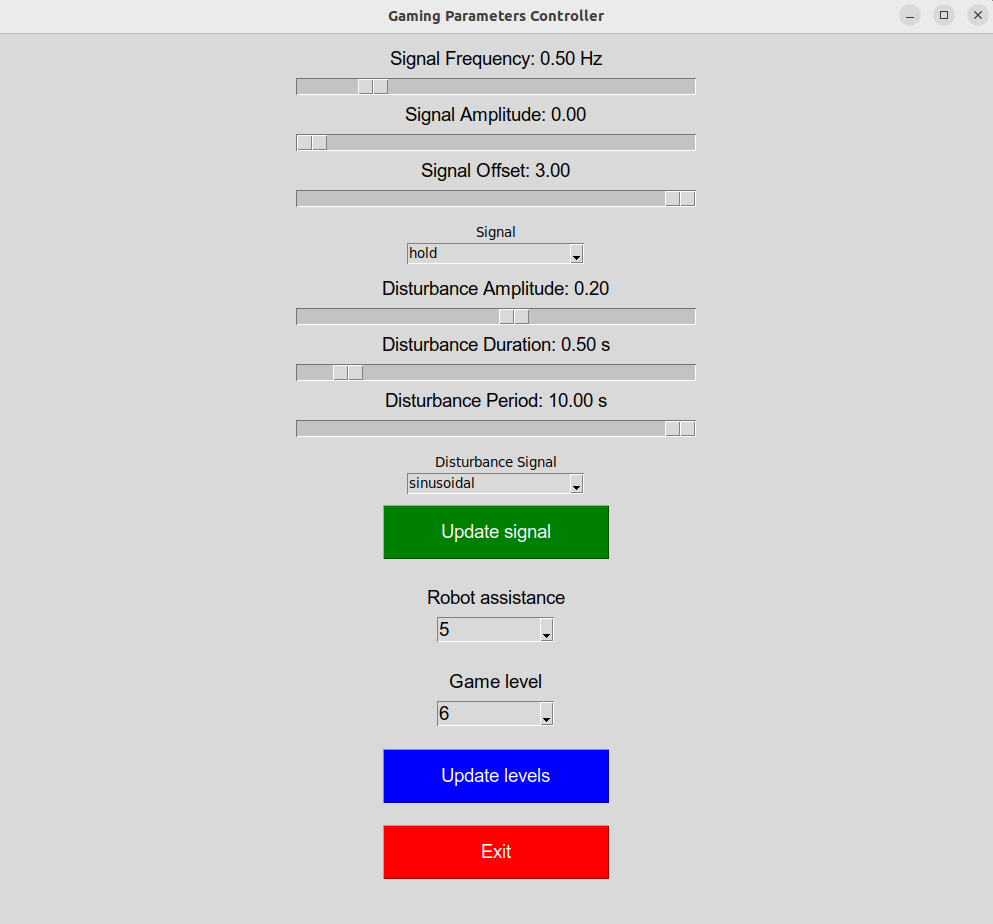
\includegraphics[width=\linewidth]{figs/control_pannel.png}
	\end{minipage}
	\caption[Interfaz de configuración de los parámetros terapéuticos]{Interfaz de configuración de los parámetros terapéuticos}
	\label{fig:control}
\end{figure}

La función \verb|saveconfig()| guarda la configuración actual de la GUI en el archivo CSV.
Las funciones \verb|update*()| convierten el valor del deslizador de \verb|str| a \verb|float|.
Entre ellas se destacan \verb|updatesignal()|, que actualiza los atributos del nodo y llama a \verb|saveconfig()|, que añade al final del archivo la nueva configuración, y \verb|updatelevel()|, que publica un mensaje con los datos de asistencia y nivel de dificultad del juego.
La función \verb|close()| finaliza el nodo y cierra la GUI y el método \verb|run()| inicia el bucle de eventos de Tkinter junto con \verb|spin_once()|.
\verb|loadcsv()| lee el último registro del archivo del paciente que se pasa como parámetro y devuelve los valores de frecuencia (Hz), amplitud (rad) de las señales de trayectoria y perturbación, duración (s), periodo (s) y nivel del juego.
Todos son \verb|float| excepto el último que es un \verb|int|.

\verb|main()| es la función principal y se encarga de extraer el ID del paciente desde la ruta al archivo de registro, cargar los datos de las señales y el juego desde el CSV, crear el nodo \verb|ScrollPublisherNode| con dichos parámetros e iniciar la GUI.
\verb|startgui()| es la primera interfaz que se lanza y gestiona la configuración del brazo que se va a rehabilitar y de los límites físicos del robot a través de la publicación de un \verb|Int32MultiArray| que actúa como un booleano indicando el botón que se ha pulsado (resetear, mínimo, máximo u offset).
El offset corresponde a la posición inicial desde la cual comienza la terapia.
Además, comprueba que se ha seleccionado o bien brazo derecho o izquierdo y que los límites mínimo y máximo se han definido correctamente antes de permitir establecer el offset o continuar a la siguiente ventana.
La decisión de ajustar los límites y el offset mediante el movimiento del brazo robótico a una posición específica, y luego guardar dicha posición a través de un botón, responde a un requisito explícito del cliente.
En la Imagen \ref{fig:config} se muestra el formato de la ventana de inicio.

\begin{figure}[ht!]
	\centering
	\begin{minipage}{0.45\linewidth}
		\centering
		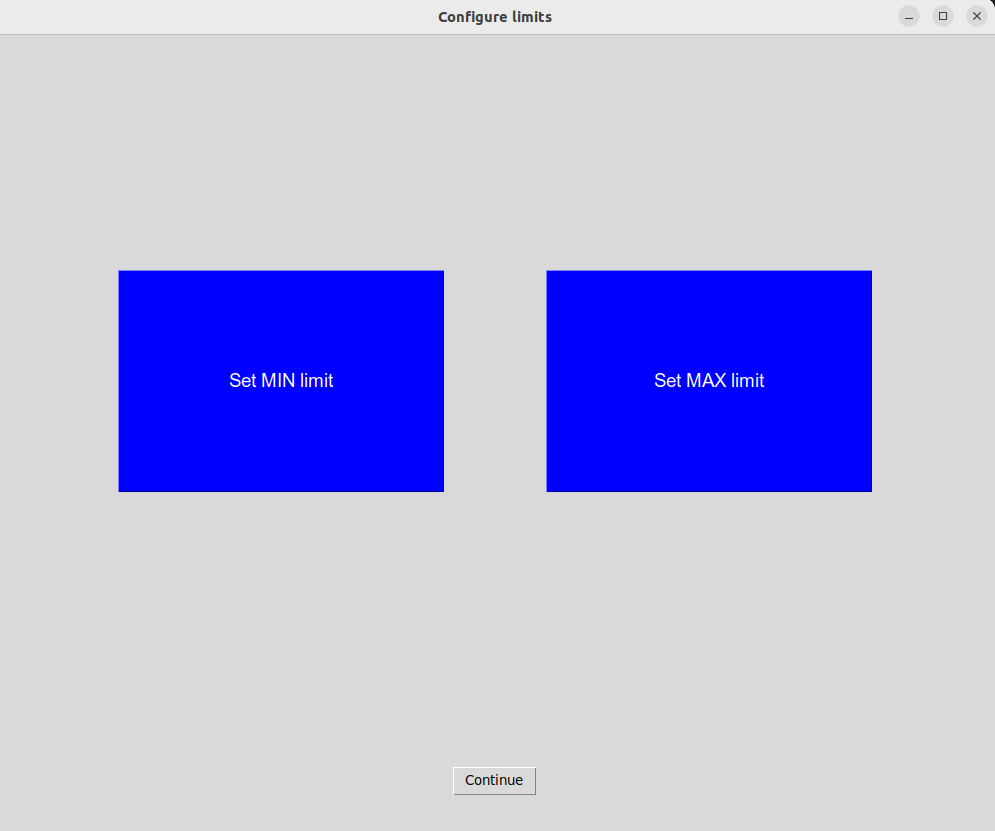
\includegraphics[width=\linewidth]{figs/config_limits.png}
	\end{minipage}
	\caption[Interfaz de configuración de los límites y orientación del brazo robótico]{Interfaz de configuración de los límites y orientación del brazo robótico}
	\label{fig:config}
\end{figure}

\section{Interfaz de visualización}
\label{section:visualization}

Este script permite observar y registrar la ejecución de un paciente en una tarea de seguimiento de trayectoria como parte de una sesión de rehabilitación motora.

Además de incluir las bibliotecas mencionadas en la Sección \ref{section:controller}, se utilizan \verb|matplotlib| para visualizar los datos del rendimiento del jugador en tiempo real, \verb|numpy| para manejar los datos de las señales que cambian con el tiempo y \verb|sys| para gestionar la ruta al archivo CSV con los datos de registro del paciente.

Se utiliza el modo interactivo de \verb|matplotlib|, \verb|plt.ion()|, que permite actualizar dinámicamente los gráficos sin bloquear el hilo principal.
Las ventanas son deslizantes respecto al eje X, no obstante debemos mantener un tamaño fijo para que la señal no se desplace hacia la izquierda, por ello se implementa \verb|np.roll()|.
El tamaño de la ventana en el eje Y se ajusta a $3$ ya que es el máximo recorrido que puede hacer el brazo.

Se define la clase \verb|FlappyBirdViewerNode| que actúa como nodo de ROS 2 y se suscribe a los topics \verb|/CleanSignal|, donde se publica la señal de referencia que se toma como trayectoria deseada que el jugador debe seguir, \verb|/Disturbance|, que contiene la señal de perturbación, \verb|/ActuatorPosition|, que publica la posición del jugador en el eje Y, y \verb|/MotorParameters|, para obtener el tiempo del juego, la posición del jugador en el eje X y el nivel de asistencia del robot.
Los mensajes de los primeros tres topics son de tipo \verb|Float32| y el último es un \verb|Float32MultiArray|.
\verb|signalcallback()| se activa cada vez que se recibe un valor de la señal, si el jugador está activo se actualizan los datos (tiempo, límites, posición, error de trayectoria y detección de colisiones) y se grafican.
Para la detección de colisiones se implementa una lógica simple basada en la comparación de la posición del jugador con los límites de la señal.
\verb|playercallback()| actualiza la posición del jugador, el offset que separa la señal de los límites y el tiempo total y marca que el jugador está activo.

En la Imagen \ref{fig:visual}, se muestran dos gráficos.
El que está en la parte superior muestra la señal de trayectoria (línea azul), la perturbación de tipo escalón (línea verde), los límites superior e inferior (líneas discontinuas grises) y la posición actual del jugador (punto rojo), proporcionando una visión clara y completa de la terapia.
Y, la parte inferior grafica el error de posición con respecto a la trayectoria deseada en función del tiempo, lo que permite detectar fallos de control, fatiga o pérdida de atención.

\begin{figure}[ht!]
	\centering
	\begin{minipage}{0.80\linewidth}
		\centering
		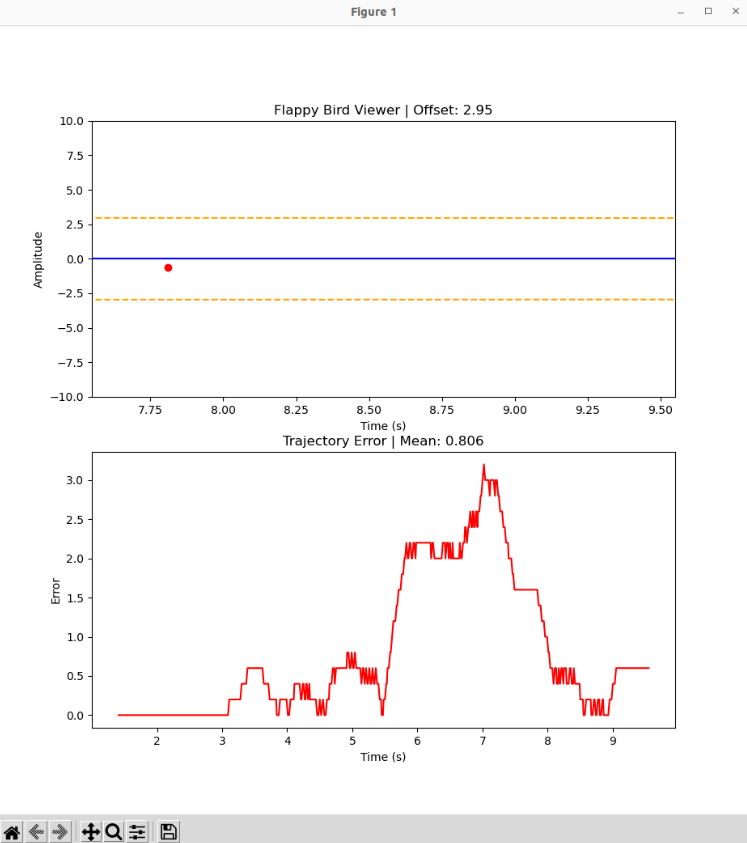
\includegraphics[width=\linewidth]{figs/visual.png}
	\end{minipage}
	\caption[Interfaz de visualización del terapeuta]{Interfaz de visualización del terapeuta}
	\label{fig:visual}
\end{figure}

En un principio, el error se calculaba en función del tiempo como se muestra en la Ecuación \ref{ec:ec1}, pero, más adelante, se optó por calcular la interpolación (o selección por índice más cercano) del valor de la trayectoria de referencia (x, y) evaluando la posición del jugador en el eje X, $x_p$, como se muestra en la Ecuación \ref{ec:ec2}.
El segundo cálculo ofrece una aproximación más precisa al error, ya que está directamente relacionado con la ubicación del jugador.
A diferencia del primer cálculo, que depende del instante de tiempo y puede verse afectado por variaciones en la sincronización de los datos.

\begin{myequation}[h]
\begin{equation}
error_t = | y_{player}(t) - y_{reference}(t) |
\nonumber
\label{ec:ec1}
\end{equation}
\caption[Cálculo del error de trayectoria en el tiempo]{Cálculo del error de trayectoria en el tiempo}

\begin{equation}
error(x_p, y_p) = | y_p - f(x_p) |
\nonumber
\label{ec:ec2}
\end{equation}
\caption[Cálculo del error de trayectoria por posición]{Cálculo del error de trayectoria por posición}
\end{myequation}

Al finalizar la ejecución, los datos más relevantes como el tiempo, la señal, los límites mínimo y máximo, la posición del jugador, el offset, el error, las colisiones y el nivel de asistencia se almacenan en un archivo CSV bajo el nombre \verb|ID-year-month-day-metrics_<index>.csv| en un subdirectorio llamado \textit{metrics} dentro del directorio \textit{home/user/database/ID/}.
\verb|index| hace referencia al número de archivo de la sesión diaria.
Esto facilita un análisis posterior de la terapia.

La función principal \verb|main()| verifica que se ha pasado como único argumento un archivo CSV con los datos de registro del paciente, extrae el ID desde la ruta, crea el nodo \verb|FlappyBirdViewerNode| y escucha de los topics.

\section{Juego flappy}
\label{section:game}

Este script implementa un juego basado en el Flappy Bird, adaptado a un entorno ROS 2 para interactuar con sensores y actuadores en tiempo real.
Existen dos modos de juego distintos, \textit{hold}, el jugador debe mantener la posición, y \textit{follow}, el jugador debe seguir una trayectoría.

Se implementan las librerías \verb|rclpy|, y \verb|std_msgs| para permitir la comunicación con ROS 2, \verb|matplotlib| y \verb|numpy| para la visualización y el manejo de señales, y \verb|pygame| para utilizar efectos de sonido.

Se emplean sonidos distintos cuando se sube de nivel, se consigue una recompensa o se colisiona.
Esto permite que el juego sea más interactivo.
En el Código \ref{cod:codejemplo3}, escrito en \textit{Python}, se observa como se carga un sonido desde un directorio, \textit{sounds}, dentro del paquete del proyecto.
Los formatos de audio más comunes soportados por \verb|pygame.mixer| son .wav, .ogg y .mp3.
La elección de utilizar la extensión .wav se debe a su simplicidad, alta calidad y compatibilidad con todos los sistemas.

\begin{code}[h]
\begin{lstlisting}[language=Python]
pygame.mixer.init()
level_up_sound = pygame.mixer.Sound('../sounds/level_up.wav')
\end{lstlisting}
\caption[Cargar un sonido al juego]{Cargar un sonido al juego}
\label{cod:codejemplo3}
\end{code}

La clase \verb|FlappyBirdNode| engloba la lógica del programa.
En \verb|__init__| se crean los suscriptores \verb|/CleanSignal|, de tipo \verb|Float32|, es la señal de referencia, \verb|/Disturbance|, también \verb|Float32|, es la perturbación, \verb|/GameParameters|, es un \verb|Int32MultiArray|, contiene el nivel del juego y de asistencia del robot, \verb|/SliderParameters|, \verb|Float32MultiArray|, para obtener el offset entre la señal y los límites superior e inferior, y \verb|/ActuatorPosition|, es un \verb|Float32|, contiene la posición del jugador en el eje Y.
Se crea un publicador \verb|Float32MultiArray|, llamado \verb|/MotorParameters|, que contiene la marca de tiempo de la ventana, las referencias de la señal y la perturbación en $(x_p, y)$, la posición del jugador en el eje X y la asistencia actualizada.
Se crea una ventana gráfica de tamaño $2x3$, donde 3 es el recorrido máximo del brazo.
En ella se representan la señal principal, los límites mínimo y máximo, las perturbaciones, la posición del jugador y objetos como estrellas y asteroides que forman parte de la lógica del juego.

La posición del jugador se representa como un punto rojo que cambia de color según la distancia a la que se encuentra entre la trayectoria deseada y los límites (negro significa que está cerca de la trayectoria, gris que está a una distancia media y rojo indica peligro de colisión con los límites).
La posición se representa como una coordenada en los ejes XY, en el eje X permanece siempre a la misma distancia (a $0,25$ unidades del origen), y en el eje Y se muestra la posición que se recibe del sensor de posición del motor.
En un principio, para validar el movimiento del jugador, la posición en el eje Y se basaba en el manejo de las flechas arriba y abajo del teclado.
Para ello se utilizó la librería \verb|pynput|.
En el Código \ref{cod:codejemplo4}, escrito en Python, se muestra la lógica de las teclas.

\begin{code}[h]
\begin{lstlisting}[language=Python]
def on_press(self, key):
	try:
		direction = -1 if self.inverted_gravity else 1
		if key == keyboard.Key.up:
			self.player_y += 0.1 * direction
		elif key == keyboard.Key.down:
			self.player_y -= 0.1 * direction
	except:
		pass
\end{lstlisting}
\caption[Movimiento vertical del jugador]{Movimiento vertical del jugador}
\label{cod:codejemplo4}
\end{code}

El método \verb|updatelevel()| cambia los colores del fondo y de la línea según el nivel, reproduce el sonido de subida de nivel y disminuye la asistencia para que la dificultad sea progresiva.
La asistencia del robot se disminuye utilizando la Fórmula \ref{ec:ec3}.
Se utiliza el máximo entre 0 y el valor calculado según el nivel para que la asistencia no sea un valor negativo.

\begin{myequation}[h]
\begin{equation}
assistance = max(0, assistance - (level - 1) // 2)
\nonumber
\label{ec:ec3}
\end{equation}
\caption[Cálculo del nivel de asistencia según el nivel de dificultad]{Cálculo del nivel de asistencia según el nivel de dificultad}
\end{myequation}

Para crear un juego dinámico que capte la atención del paciente se crea una misión secundaria en cada nivel.
Los niveles 1, 4 y 7 tienen como objetivo permanecer dentro de los límites por un tiempo determinado.
Esto permite evaluar la precisión del paciente.
Además, cuando se sobrepasa uno de los límites el contador se para y se reanuda de nuevo cuando se vuelve al camino.
Los niveles 2 y 6 se enfocan en el ajuste de la posición para chocar con las estrellas que están dispuestas en la señal principal.
De esta forma se consigue que el paciente permanezca y siga la trayectoria deseada.
Los niveles 3 y 8 pretenden ejercitar la rapidez de reacción mientras el paciente evita colisionar con los asteroides.
Los niveles 5 y 9 fomentan la flexibilidad cognitiva del paciente para adaptarse a una nueva lógica de control basada en el concepto de gravedad invertida (arriba es abajo y viceversa).
Y, por último, el nivel 10 permite al médico evaluar distintos escenarios límites mediante ajustes en los parámetros de la señal, perturbación y el offset.
En las Imágenes \ref{fig:level} y \ref{fig:level2} se comparan dos niveles diferentes del juego.
La primera imagen presenta límites más estrictos que la segunda, que se han coloreado para que se vean claramente en el estudio, pero en el juego son dos líneas de color blanco punteadas para evitar distracciones del paciente.
En la segunda imagen, se observan dos perturbaciones de tipo sinusoidal con sentidos opuestos, representadas por triángulos verdes cuya punta indica el signo de la perturbación.
Si fuese una perturbación de tipo escalón, los triángulos se pintan de color naranja siguiendo la misma lógica de graficación.
En contraste, la primera imagen no muestra ninguna perturbación.

\begin{figure}[ht!]
	\centering
	\begin{minipage}{0.85\linewidth}
		\centering
		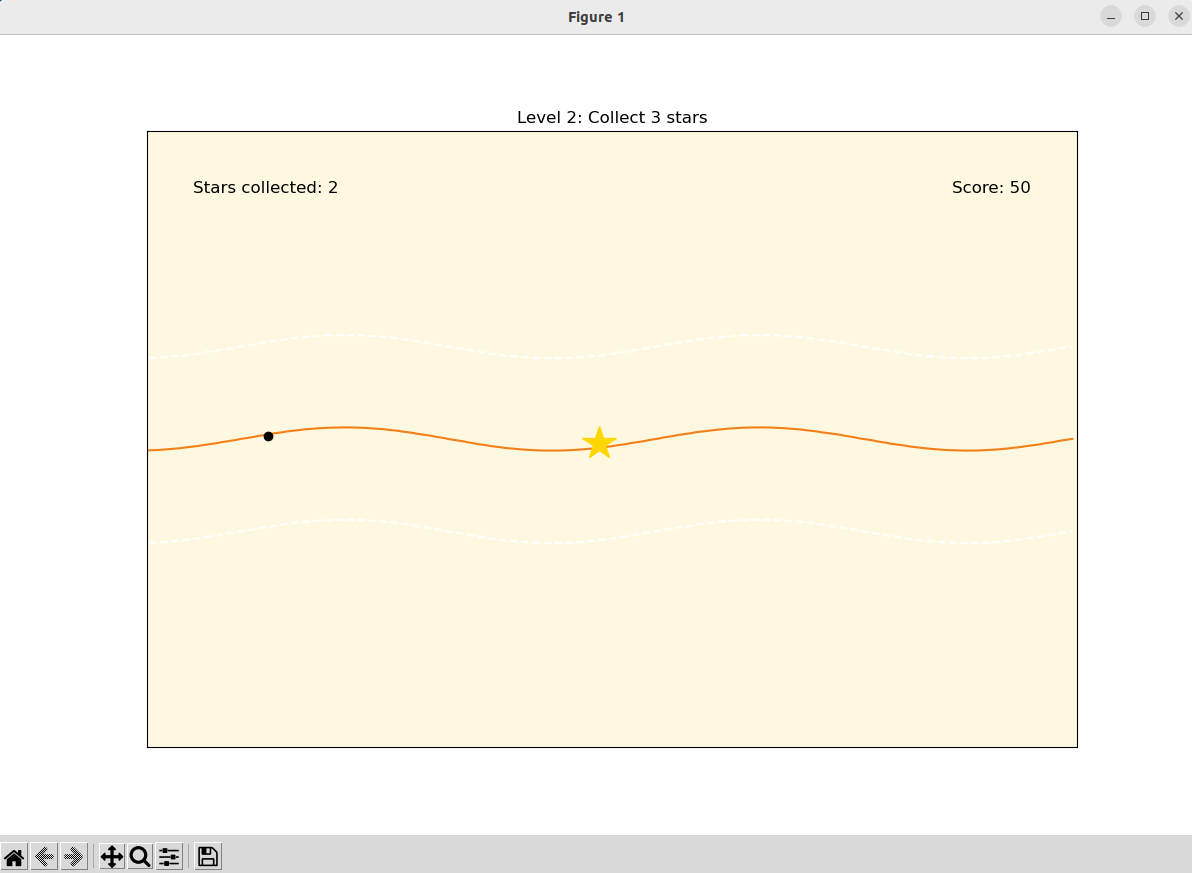
\includegraphics[width=\linewidth]{figs/flappy_level.png}
	\end{minipage}
	\caption[Nivel 2 del juego sin perturbación]{Nivel 2 del juego sin perturbación}
	\label{fig:level}
\end{figure}

\begin{figure}[ht!]
	\centering
	\begin{minipage}{0.70\linewidth}
		\centering
		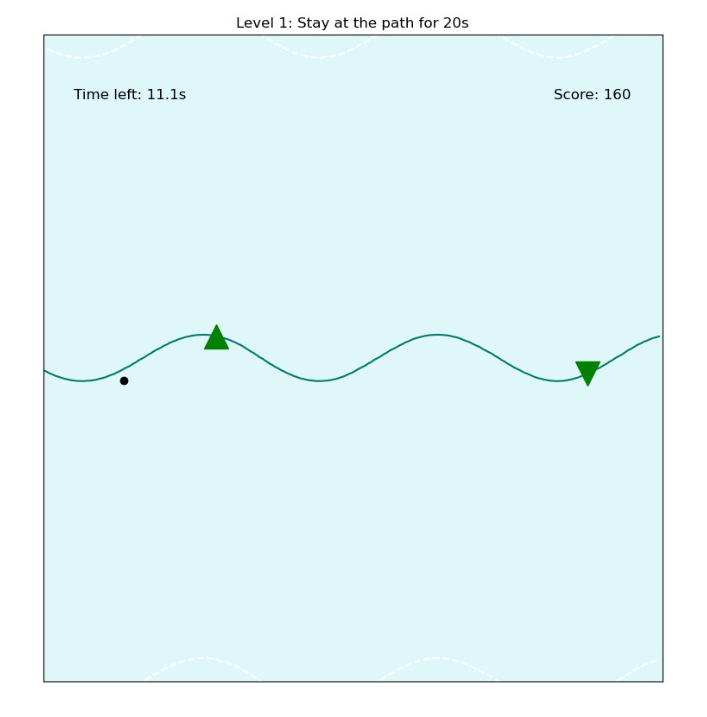
\includegraphics[width=\linewidth]{figs/flappy_level2.png}
	\end{minipage}
	\caption[Nivel 1 del juego con perturbación]{Nivel 1 del juego con perturbación}
	\label{fig:level2}
\end{figure}

Se introduce un sistema de recompensas para aumentar la motivación y destreza del paciente.
Esto permite reforzar comportamientos y habilidades específicas para alcanzar los objetivos propuestos.
Cada vez que se consigue una estrella y se sube de nivel se suman 10 y 30 puntos, respectivamente, a un contador.
Y, cuando se colisiona con un asteroide, el contador decrementa en 5 puntos.
Para ello se utilizan las funciones \verb|incrementscore()| y \verb|decrementscore()|.

Los objetos como las estrellas, los asteroides y los triángulos, que indican el sentido y comienzo de una perturbación, se crean con \verb|ax.plot|.
Las estrellas se generan de forma aleatoria en el eje X, y los asteroides en ambos ejes con límites definidos entre $(0.3, offset)$ y $(-offset, -0.3)$.
El máximo de objetos visuales al mismo tiempo dentro de la ventana es 2.
Las funciones \verb|generatestar()|, \verb|generateasteroid()| y \verb|generatedisturb()| encapsulan la lógica de creación de objetos, y la función \verb|clearobjects()| la eliminación de estos.

El desarrollo del juego está concentrado en \verb|listenercallback()|, que es el bucle principal y se ejecuta cada vez que se recibe un nuevo dato en el topic \verb|/CleanSignal|.
Se utilizan las funciones \verb|np.roll| y \verb|plt.ion()| de las bibliotecas \verb|NumPy| y \verb|Matplotlib|, respectivamente.
\verb|np.roll| actualiza la señal y la perturbación.
Como se explica en la Sección \ref{section:visualization}, los gráficos se actualizan en tiempo real con \verb|plt.ion()|.

Los callbacks actualizan los datos que se reciben de los topics, estas funciones son \verb|disturbcallback()|, \verb|levelcallback()|, \verb|offsetcallback()| y \verb|positioncallback()|.

La función \verb|main()| inicializa el nodo ROS, crea una instancia del juego y entra en un bucle hasta que el usuario detenga el programa.\\

El proyecto es fácilmente escalable en el caso que se quiera añadir una señal que sea combinación de otras.
Simplemente se debe obtener la señal del topic \verb|/CleanSignal| si es de tipo trayectoria o de \verb|/Disturbance| si es de tipo perturbación.
En cuanto a la selección de esta nueva señal, es suficiente con incluir una nueva opción dentro de la \verb|Combox| a la que hace referencia.
